\documentclass[30pt,landscape,magscalefonts]{foils}
\usepackage{floatflt}
%\usepackage{times}
\usepackage{tabularx}
\usepackage[pdftex]{graphicx}
\graphicspath{{./graphics/}}
\usepackage[pdftex]{color}
\usepackage[pdftex]{geometry}
\geometry{headsep=2.0em,hscale=0.80}
\usepackage{hyperref}
\hypersetup{
  pdftitle={SDR 2003 Report on Player},
  pdfauthor={Brian P. Gerkey, USC Robotics Research Lab},
  pdfpagemode={FullScreen},
  pdfborder={0 0 0}
}
%\usepackage{background}

% define some nice colors
\definecolor{myred}{rgb}{0.6,0,0}
\definecolor{myblue}{rgb}{0,0.2,0.4}
% set default background and text colors
%\pagecolor{white}
\color{myblue}

% don't want any paragraph indentation
\setlength{\parindent}{0cm}

% wrapper for foilhead that sets the text color
\newcommand{\foilheadc}[1]{\foilhead{\Large \textcolor{myred}{#1}}\vspace*{-2em}}
% wrapper for itemize that shortens the inter-item separation
\newenvironment{xitemize}{\begin{itemize} \itemsep 1pt}{\end{itemize}}
% wrapper for enumerate that shortens the inter-item separation
\newenvironment{xenumerate}{\begin{enumerate} \itemsep 1pt}{\end{enumerate}}

\def\movieroot{file:///mnt/win/users/gerkey/videos}

\title{\textcolor{myred}
{\large The Player/Stage Project: Current Status and Future
Directions\vspace*{1em}}}
\author{\small Brian P. Gerkey\hspace{1.5em} Richard T. Vaughan\hspace{1.5em}
Andrew Howard\vspace*{1em}\\
\includegraphics[height=15mm]{cres-logo.jpg}
\includegraphics[height=15mm]{usclogo.jpg}\hspace*{2em}
\includegraphics[height=15mm]{hrl_logo.jpg} \vspace*{1em}\\
{\tt \small http://playerstage.sourceforge.net}}
\date{}

% headers, etc.
\rightheader{
\includegraphics[height=15mm]{cres-logo.jpg}
\includegraphics[height=15mm]{usclogo.jpg}
}
\leftheader{\includegraphics[height=15mm]{hrl_logo.jpg}}
\MyLogo{}
\def\totalpages{\pageref{lastpage}}
\rightfooter{\textcolor{myblue}{\quad\textsf{\thepage/\totalpages}}}

\begin{document}

% the title slide
\maketitle

% get the page numbering right
\pagebreak\setcounter{page}{2}

\MyLogo{\textcolor{myblue}{SDR PI Meeting, March 2003}}

\foilheadc{Project overview}
The Player/Stage project is a collaborative development effort aimed at
producing high-quality open-source tools for robotics researchers.

\vspace{1em}
The project primarily maintains two pieces of software:
\begin{itemize}
\item {\bf Player}: A networked robot device server.
\item {\bf Stage}: A multiple robot simulator.
\end{itemize}

\foilheadc{Usage}
\begin{center}
\includegraphics[height=130mm]{usage-map.jpg}
\end{center}

\foilheadc{Usage (cont'd)}
\begin{center}
\includegraphics[height=130mm]{stats_graph_blur.jpg}
\end{center}

\foilheadc{Supported hardware / software}
{\small
\begin{itemize}
\item {\bf Robots}: ActivMedia, RWI, K-Team
\item {\bf Lasers}: SICK LMS 200
\item {\bf PTZ}: Sony EVID30
\item {\bf IMUs}: Microstrain 3DM-G IMU, ISense InertiaCube2
\item {\bf Wifi}: linuxwifi, iwspy, aodv
\item {\bf Vision}: ACTS, CMVision
\item {\bf Speech}: Festival
\end{itemize}
}

\foilheadc{Player architecture}
\begin{center}
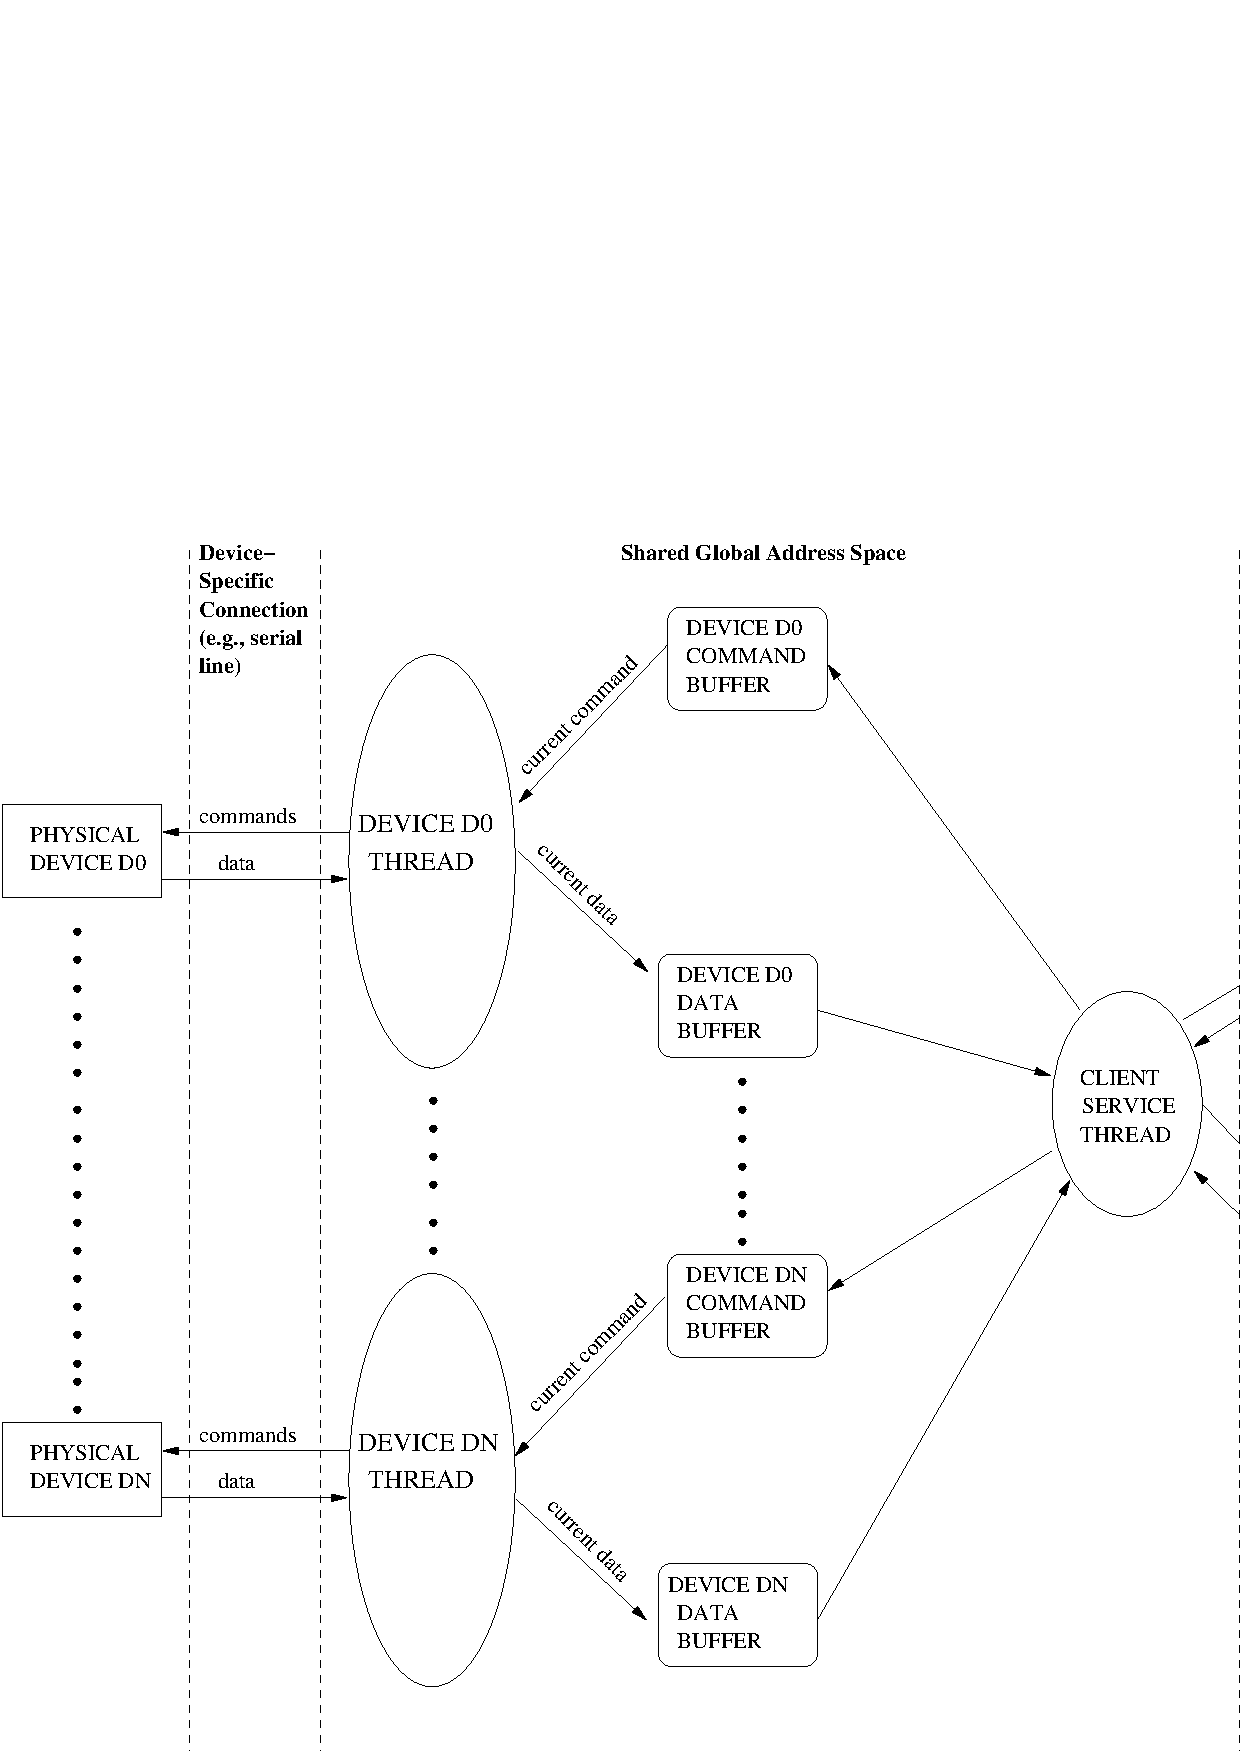
\includegraphics[height=130mm]{buffers.pdf}
\end{center}

\foilheadc{Player design}
Player is built on 3 key abstractions, borrowed from operating systems
design:

\begin{tabular}{cc}
\parbox{.6\textwidth}{
\begin{itemize}
\item read/write/ioctl model
\item \fbox{interface/driver model}
\item client/server model
\end{itemize}}
&
\parbox{.3\textwidth}{\includegraphics[width=.3\textwidth]{pioneer-2-small.jpg}}
\end{tabular}

\foilheadc{Interfaces vs.\ drivers}
\begin{xitemize}
\item A device {\em interface}, such as {\bf sonar}, is a generic
specification of the format for data, command, and configuration
interactions.
\item A device {\em driver}, such as {\bf pioneer-sonar} or {\bf
rwi-sonar}, specifies how the low-level device control will be carried
out.
\item Multiple drivers can present the same interface.
\item The {\bf same} controller can be used with {\bf different} devices.
\end{xitemize}

\foilheadc{Sophisticated drivers}
\begin{itemize}
\item Drivers can do much more than provide transparent access to a device.
\item Arbitrary computation can be embedded in a driver.
\item Well-understood algorithms can be encapsulated in Player and
offered as standard services.
\item Examples: acoustic filtering, probabilistic localization.
\end{itemize}

\foilheadc{Sophisticated drivers (cont'd)}
The {\bf laser-visual fiducial-finder}:

\begin{tabular}{cc}
\parbox{.7\textwidth}{
\begin{itemize}
\item Uses laser range-finder, PTZ camera and color segmenter to locate and 
identify fiducials.
\item Performs sensor fusion on range and image data.
\item Includes closed-loop control of PTZ camera.
\end{itemize}}
&
\parbox{.3\textwidth}{\href{\movieroot/lvb.avi}{\includegraphics[width=.21\textwidth]{laservisualbeacon2.jpg}}}
\end{tabular}

\foilheadc{Shifting the computation}
\begin{xitemize}
\item When an algorithm is implemented as a driver, the associated
computational load is moved to the server.
\item The {\bf passthrough} driver acts as a proxy within one server
for a device in another server.
\item Allows computational load to be shifted arbitrarily, within a
network or across the Internet.
\item Also allows one server to aggregate and distribute data and
commands for multiple robots.
\end{xitemize}

\foilheadc{Relevance to SDR-II}
{\small
\begin{xitemize}
\item All Player/Stage software is Open Source, released under the GPL.
\item Player runs on many OSs (e.g., Linux, Solaris, OS~X, FreeBSD)
\item Player runs on many embedded systems 
(e.g., ipEngine, nanoEngine, XScale, iPAQ).
\item Player supports many common research robots, including the AmigoBot.
\item Player and/or Stage already used within SDR.
\end{xitemize}
}

\foilheadc{Accomplishments}
Added to the server:
\begin{itemize}
\item Synchronous request/reply mechanism.
\item Distributed computation.
\item Laser-based feature detectors.
\item Beacon-based localization.
\item Map-based localization using particle filters.
\end{itemize}

\foilheadc{Player future work}
\label{lastpage}
\begin{xitemize}
\item Simultaneous localization and mapping.
\item Device name-server / discovery.
\item More closed-loop control:
\begin{xitemize}
\item Impedence controller
\item Target-tracking (visual servoing)
\item Waypoint-following
\item Wall-following
\item Formation-maintenance
\end{xitemize}
\end{xitemize}

\end{document}
